\chapter[Results and future developments]{Results and future developments}

\section[Measurements summary]{Measurements summary}

\subsection[Input power levels]{Input power levels}

A number of measurements have been collected during 2016. Figure \ref{g_IP} shows the relation between the average gradient and the input power in the accelerating structure. The measurement points have been selected to allow the comparison between the different running conditions, as outlined in Chap. \ref{chap:motivation}, and are summarised in Table \ref{run_pwr}.

\begin{table}
  \centering
    \begin{tabular}{ c l }
    \hline
    \hline
    Run type		&	Input power (MW)		\\
    \hline
    unloaded 		&	43.3, 41, 38 and 24.6	\\
    loaded			&	43.3, 41 and 38			\\
    anti-loaded		&	6.5					\\
    \hline
    \hline
    \end{tabular}
\caption{Input power levels of measurements in 2016.}
\label{run_pwr}
\end{table}

The measurements at different input power level have not been taken in a precise order, anyway it has been tried to keep long measurement periods as much as possible at the same input power. 
The choice is normally complicated by the fact that the Xbox was not able to provide the maximum RF power level during the year, mainly because of technical problems. The order of the runs at constant input power is reported in Fig. \ref{BDR ALL, in appendix ???}.


\subsubsection{Comparison of loaded and unloaded runs at same average gradient}

For the CLIC test purpose,  carry out a measurement at 100 MV/m average gradient comparing loaded and unloaded runs would be the most interesting measurement possible. In order to perform it, the input power has to raised from 43.3 MW in the unloaded case to 67.5 MW in the loaded case. 

Unfortunately it was clear from the beginning that reaching 67.5 MW of input power was not possible because the waveguides that deliver the power from the pulse compressor to the structure under test are not conditioned for such high power flux.

Because of this limitation, the choice comes down to perform measurements at the same input power and compare the results. 

During a period of technical problems, it has been anyway collected an unloaded measurement at 24.6 MW of input power, in order to compare it with the correspondent average gradient in the loaded case at 43.3 MW of input power. Unfortunately with a such low input power, the breakdown rate is very low, and after 4 days of measurements zero breakdowns were collected. Therefore it is only possible to affirm that running unloaded at 24.6 MW input power, the breakdown rate is $< 7.7 \, 10^{-8} $ BD pulse$^{-1}$. 


\subsubsection{Comparison of loaded and unloaded conditions at same input power}

Most of the measurements carried out during 2016 campaign were comparing the loaded and unloaded running condition. The input power levels used were 43.3, 41 and 38 MW. It was not possible to go at lower input powers because the breakdown rates becomes so low that the data collection takes weeks to produce a sufficient statistics.


\subsubsection{Study of the antiloaded runs}

The antiloaded measurements were carried out at 6.5 MW of input power. The reason is that with a beam current  of 1.6 A, the output gradient of the structure is already around 100 MV/m (see Fig. \ref{3grad}). The results were indeed interesting and will be shown later when it comes to talk about the breakdown distribution.




\begin{figure}[t]
\centering 
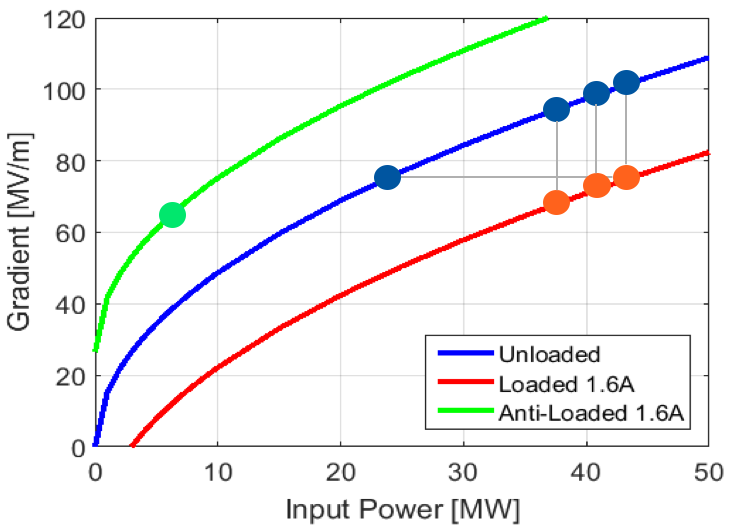
\includegraphics[scale=0.7]{pictures/grad_vs_inPow.png}
\caption{Average gradient as function of the input power in different running conditions. See text for details on the measurement points. }
\label{g_IP}
\end{figure}


\subsection[Beam pulse parameters]{Beam pulse parameters}

As mentioned in the motivation of the experiment, the goal is to understand the effect of the beam on the breakdown rate. The beam parameters have been therefore selected in order to enhance the effect of the beam, rather than try to simulate the CLIC operation. This materialises in:
\begin{itemize}
\item Higher beam current than CLIC: 1.6 A instead of 1.2 A.
\item Longer beam pulse: the beam is lasting during all the compressed RF pulse, for 250 ns, instead of last just during the flat-top of the CLIC pulse (see Sec. \ref{sec:PCtune}).
\end{itemize}

\noindent
The loaded operation is clearly visible  in the RF signals, as shown in Fig.~\ref{RF_load}.

\begin{figure}[h]
\centering
  \subfigure[Loaded operation]
   {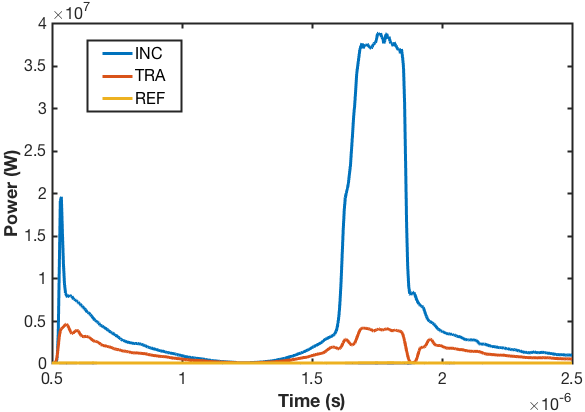
\includegraphics[scale=0.33]{pictures/LoadedPulse.png}}
  \subfigure[Antiloaded operation]
   {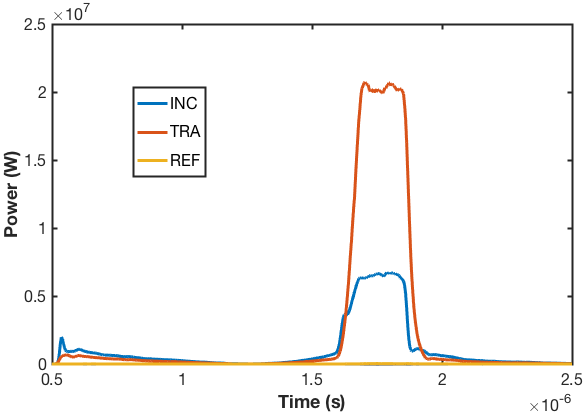
\includegraphics[scale=0.33]{pictures/AntiloadedPulse.png}}
\caption{Comparison of the RF signals during the loaded and antiloaded operation. During the loaded operation it can be observed that the transmitted power falls close to zero, because of the energy subtracted from the beam. The opposite behaviour can be noted in the antiloaded case, where the input power is much lower than the transmitted. In this case the difference in energy is provided by the beam, that gets slowed down because of the wrong phase with the RF. }
 \label{RF_load}
 \end{figure}




\section[Breakdown rate measurement results]{Breakdown rate measurement results}



\section[Breakdown distribution]{Breakdown distribution}

\subsection[A model for the breakdown distribution]{A model for the breakdown distribution}

Unloaded experiments exhibit a flat distribution of the breakdowns in the accelerating structure. In addition, it is known that the breakdown rate follows the scaling law in Eq. \ref{E30}, but it has been derived from the data available from the unloaded tests as well. From these considerations arises the necessity to understand if these results are still valid when running with the beam inside the accelerating cavity.

Considering any cell as a substructure, it is reasonable suppose that cells with a higher accelerating field will be more likely to experience breakdowns than cells with a lower field. According to this reasoning and following the Eq. \ref{E30}, the breakdown probability per cell is given by
\begin{equation}
\text{BD probability (\%)} =\frac{   \left ( \frac{E_\text{cell}}{E_\text{max}} \right )^{30} }{ \sum \left( \frac{E_\text{cell}}{E_\text{max}} \right )^{30}   }
\end{equation}
where E$_\text{cell}$ is the surface electric field in the centre of the cell and E$_\text{max}$ is the maximum surface electric field at the centre of a cell. 

The choice of using the surface electric field instead of the accelerating gradient comes from the physics of the breakdown process \cite{Walter:PC}. Anyway the shape of the gradient profile and of the surface electric field along the structure differs only slightly. The field of the coupling cells is assumed as the same in the adjacent cells. This comes from geometrical considerations, and could be eventually derived from simulations \cite{Alexej:PC}.

The result is shown in Fig. \ref{BD_prob}. The expectation is to have a almost flat distribution in the unloaded case, with and accumulation of the number of breakdowns in the first part of the structure for the loaded case and at the end of the structure for the antiloaded case.


\begin{figure}[h]
\centering 
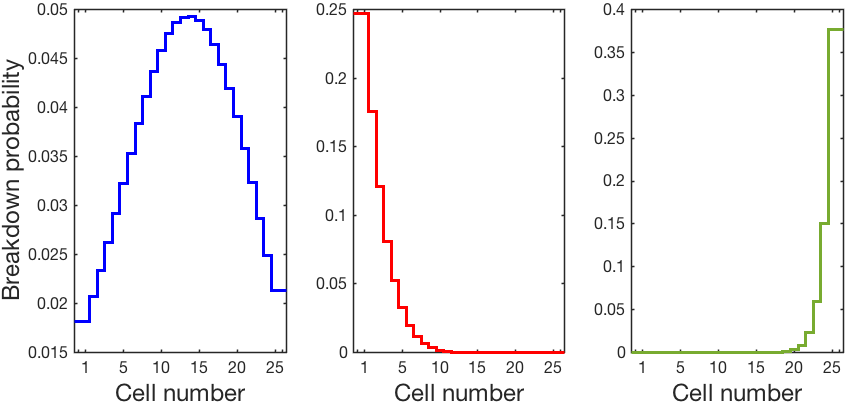
\includegraphics[scale=0.45]{pictures/BD_probability.png}
\caption{Breakdown probability according to the model in different running conditions: unloaded (left), loaded (center), antiloaded (right). The different scale has to be noted: while the breakdown probability oscillates between the 1.8\% and 5\% in the unloaded case, when the beam is present the difference is much bigger.}
\label{BD_prob}
\end{figure}


\subsection[Measurement results]{Measurement results}

The breakdown distribution, cumulating the data at the same input power, are shown in Fig. \ref{BD_distro}. Both the linear scaling with the surface field and the scaling proposed in the precedent section are plotted.


\begin{landscape}


\begin{figure}[h]
\centering 
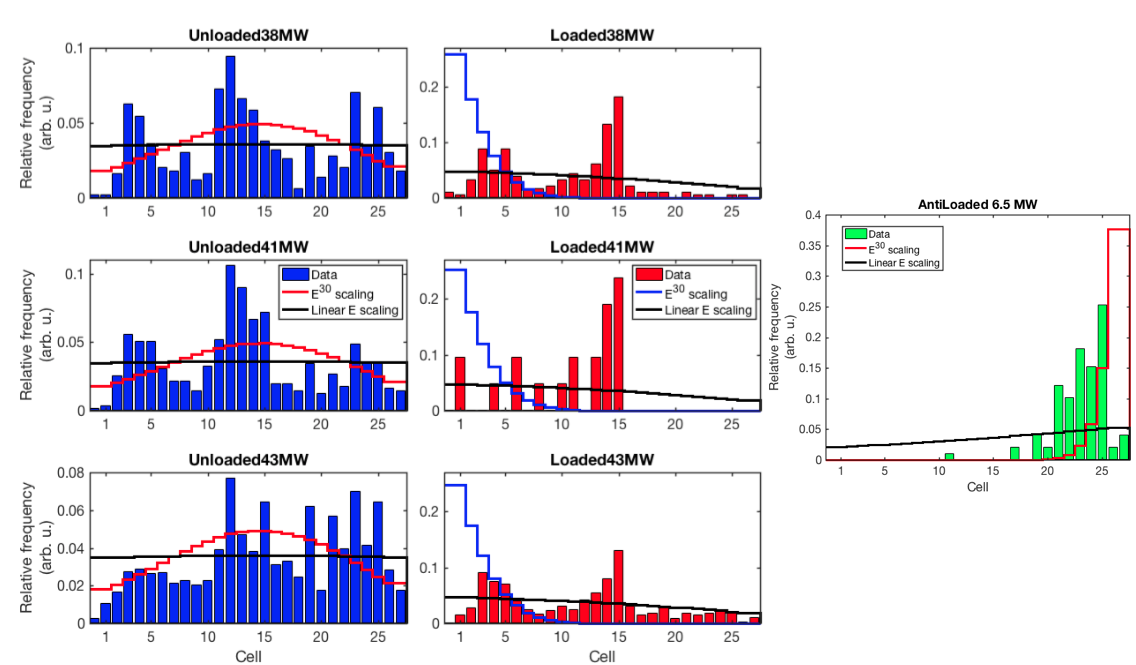
\includegraphics[scale=0.53]{pictures/distro_all.png}
\caption{Measured breakdown distribution in the accelerating cavity under test in different running conditions. Over the data is plotted the proposed scaling and the linear scaling with the surface field is plotted (in black).}
\label{BD_distro}
\end{figure}

 
\end{landscape}







\section[Beam induced RF]{Beam induced RF}






\section[Further developments]{Further developments}


RF:
- TWT already eliminated (no spikes anymore)
- I suggest to switch the pulse compressor to a SLED-II type, which is more stable, avoiding all the tuning problems we had
- ?


\section{Conclusions}

During the measurement campaign of this year we learnt how to operate and measure the breakdown rate of the structure with and without beam.

The beam effect analysis has still to be carried on in detail, in particular have to be understood if when running with beam the conditioning takes place or not. Further investigations on this topic require a stable and extensive beam time, which was not the case of the CTF. The comparison of this data with the ones of a stable long test with beam can suggest that switching condition ripetutamente w/ w/o beam can lead to a higher BDR ...
- as DC tests suggest
- as we cannot see because of the low rep.rate



shown effect on the migration !